%File: formatting-instruction.tex
\documentclass[letterpaper]{article}
\usepackage{aaai}
\usepackage{times}
\usepackage{helvet}
\usepackage{algorithm}
\usepackage{algpseudocode}
\usepackage{courier}
\usepackage{graphicx}
\graphicspath{{./figure/}}
\frenchspacing
\setlength{\pdfpagewidth}{8.5in}
\setlength{\pdfpageheight}{11in}
\pdfinfo{
/Title (Multiple Object Tracking using Spatial Reasoning)
/Author (Xiaoyu Ge, Jochen Renz)}
\setcounter{secnumdepth}{0}  
 \begin{document}    
\begin{abstract}
Intelligent agents perceive the world mainly through images captured at  different time points. Being able to track objects from one image to another is fundamental for understanding the changes of the world. 
Humans can perform efficient object tracking by common sense reasoning. For example, we know that a free falling object will not change its downwards movement unless acted upon by another force. Given an initial image with a free falling object, we will first check the objects which are below the initial object location in order to find the corresponding object in subsequent images. 

Object tracking has been extensively studied within the context of computer vision. However, reasoning is typically not used to solve this problem. Most tracking algorithms represent and track objects by their visual features and trajectories. Those algorithms become error prone when there are multiple objects with the same appearance that follow similar trajectories, that change trajectories, or when trajectories are not available. 

In this paper, we propose a solution to the problem of tracking multiple objects across images taken at different time points. We represent objects using general solid rectangles, i.e., rectangles that can have any angle and are not penetrable (GSRs). GSRs are often used in computer vision and video games. We present a modified version of the GR-n representation [Ge and Renz, IJCAI 2013] that allows us to specify useful spatial constraints and infer possible spatial changes of GSRs. 

Our solution is closer to human reasoning in that it considers spatial relations and physical properties of objects. It can improve tracking accuracy significantly by qualitatively predicting possible motions of objects and discarding matches that violate spatial constraints. 

We evaluate the solution in a real video gaming scenario. We capture sequences of screenshots of the game where multiple objects are moving, and compare the tracking accuracy by varying the length of the intervals between the time points at which the screenshots are taken. We also show that our solution can be extended with more powerful qualitative reasoning models to tackle multiple object tracking when the time interval between images is long. 
\end{abstract}
\section{Introduction}

Visual perception is one of the main sources of information about the world. Most intelligent agents have eyes, cameras, or other optical devices to "see" their environment and to detect changes in their environment. The information these devices provide is in the form of image sequences, or if the image sampling rate is high enough, we call it video.
Image understanding \cite{sridhar_video_2011} and object detection \cite{papageorgiou1998general} are essential methods for extracting useful information from images. Equally essential is object tracking \cite{yilmaz2006object}, that is the ability to identify the same object in a series of images or in video and to track its movement and its changes. Existing object tracking methods typically rely on the visual appearance of objects and on their trajectories to successfully track even temporarily occluded objects \cite{}.
Similar methods are used for multiple object tracking \cite{}.
In this paper we are interested in a problem that can occur when intelligent agents observe the world through visual perception and have to track changes.
It can be described as follows: Given two images, let's call them "before" and after", that depict the same scene at different times. Between the two images, certain physical actions have been happening that affected the locations and possibly the states of the objects in the scene. Our task is to find a match between the objects in the "before" image with the objects in the "after" image that is consistent with the effects of the physical actions that happened between the two images. In case there are multiple consistent matches, we want to identify the most plausible one.

It is clear that this problem is relatively straightforward to solve if the visual appearance of all objects in each image is unique, as we simply match the objects that have the same visual appearance. The problem gets challenging, if multiple objects have the same visual appearance. We say that objects of the same visual appearance have the same type and we can only match objects of the same type. Whenever there are multiple objects of the same type, existing object tracking methods are not applicable any more.

There are different variants of this problem depending on the way the relevant physical actions are specified or unspecified. In general, the actions pose additional constraints that have to be satisfied. These constraints can vary from case to case and typically depend on the application. One variant of the problem is when the specific actions that are responsible for the changes are unknown. Then the task is to find a match for which (THIS IS REALLY WEIRD THAT WE DO NOT TAKE INTO ACCOUNT THE PARTICULAR ACTION!!!) the standard laws of physics are satisfied. ARE WE REALLY DOING THIS, DOES THIS MAKE SENSE?
We could also formulate the problem as identifying physical actions that explain a given match.
Depending on the speed of the changes, it is clear that the longer the time gap between the "before" and the "after" image, the less accurate a match might be.

There are many real-world situations where this problem occurs. For example in natural disasters such as earthquakes, storms, or tsunamis, where we often see before and after images, also in terrorist attacks or bomb explosions. But there are also less dramatic situations, for example a satellite that takes another image of the same site at the next fly-over.

Our interest in this problem is motivated by the Angry Birds AI competition where the task is to build an AI agent that can play Angry Birds as good as the best human players. One major problem in this context is to be able to accurately predict the outcome of an action. To do this, we need to learn from previous cases where the effect an action had on a given scenario is known. As input to the machine learning algorithms we need to know the initial scenario, the action that was used and the effect the action had on each object in the initial scenario, i.e., we need to know exactly which object in the initial state corresponds to which object in the resulting state. In order to be able to learn a huge number of cases, we need to be able to automate the matching between objects in the "before" and in the "after" image.

We evaluate our proposed solution using the Angry Birds scenario. We take two subsequent screenshots of an active Angry Birds game with varying time gaps and apply our method to match the objects between the two screenshots. We measure the accuracy of our method by using the percentage of correct matches out of the total number of possible mismatches. As expected, it turns out that the smaller the time gaps, the higher the accuracy of the matches.

 
\section{Objects Representation with the extended GSR (EGSR)}

We use a minimum bounding rectangle to approximate the region occupied by a circle and use exact shapes for the rectangles.

Since the objects can only interact via contacts, it is important to distinguish if and how two objects contact each other. A proper representation should allow us to infer possible motions of an object from its interaction with other objects. 

We use GSR\cite{} to model the contacts between solid rectangles. GSR defines eight contact sectors that correspond to the eight edges and corners of the rectangles. Given two GSRs $o_1$ and $o_2$ that contact each other via $sector_1, sector_2 \in \{S_1, ..., S_8, R_1, ..., R_8\}$, the contact relation between $o_1$ and $o_2$ can be expressed as the constraint $o_1 \, (sector_1, sector_2) \, o_2$. 

However, GSR introduces ambiguities when the rectangles are disconnected. To overcome the ambiguities, we partition the embedding space around an reference object into nine mutually exclusive tiles[cite, CDC]. The centre tile corresponds to the minimum bounding rectangle of the object and the other eight tiles correspond to the eight cardinal directions. 

Given two spatial objects, if the MBRs of the two objects intersect or boundary touch, we assign a GSR relation accordingly. Otherwise, one of the eight cardinal tiles will be used to indicate the spatial relation. The GSR relation between a pair of objects can be obtained by first calculating the distance between each pair of the contact sectors and then using the pair with the shortest distance. The distance becomes zero when the two objects touch. 

\begin{figure}[h!]
\centering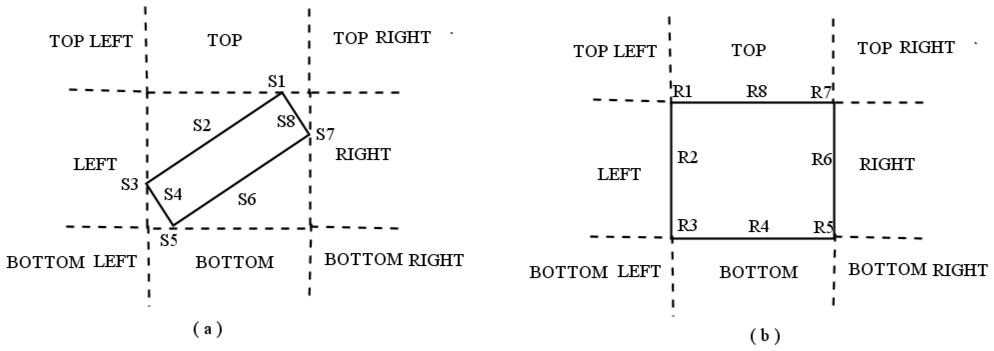
\includegraphics[scale=0.25]{EGSR-relations.png}\caption{Contact sectors and Cardinal directions of (a) an angular rectangle and (b) a normal rectangle}
\end{figure}

\section{Efficient Matching by Approximating Movement}

To find out the best matchings, a straightforward approach is to enumerate all the possibilities. The search space is huge as there is a combinatorial number of potential matches between any two object sets. However, most matches can be avoided by searching through the corresponding objects only in a limited area. The area of the initial object should therefore cover all the objects in the subsequent scene that can be potentially matched to the initial object.  We use a circular region to represent this area. The circle's centre is located at the centroid of the initial object and the radius of the circle is the maximum shift of the centroid. The radius is calculated as $V \times T$ where $V$ is the maximum velocity of the object and $T$ is the time gap between the initial and subsequent scenes. This calculation ensures that the circle can adapt to different time gaps. We call this circle the $movement\,bounding\,circle$(MBC).  

The MBC can be divided into four quadrants to further restrict the search area. A quadrant is said to be open if all the objects in that quadrant can be considered as potential matches of the referred object, otherwise the quadrant is closed. An initial object will be matched with one of the subsequent objects within the open quadrants while the others will not be considered. 

 Given a MBC $C$, the open quadrants are $C^{(i,j)}, i,j \in \{-, +, *\}$ where $(+,+)$, $(+,-)$, $(-,-)$, $(-,+)$ correspond to the top-right, top-left, bottom-left, bottom-right quadrants respectively (Figure \ref{Quadrants}.a). $(*, *)$ refers to an arbitrary quadrant. 

The relative distance between two objects can be allocated to three meaningful classes, namely touch, reachable, and non-reachable (Figure \ref{Quadrants}.b). An object $O$ can touch another object $O^\prime$ at one of its contact sectors. $O^\prime$ is reachable by $O$ if $O^\prime$ is within the MBC of $O$ otherwise non-reachable.

\begin{figure}[h!]\label{Quadrants}
\centering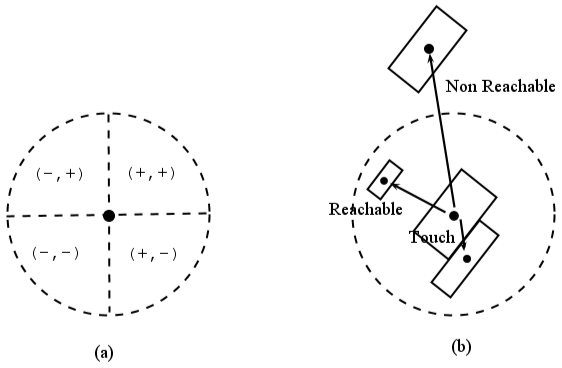
\includegraphics[scale=0.3]{quadrants.png}\caption{(a) The four quadrants of a MBC (b) Qualitative distance with respect to object A and its MBC}
\end{figure}

We can infer the open quadrants for an object by approximating the movement direction of the object, i.e. by estimating which of the quadrants the object is most likely to be in at the next time point. 

Object movement can be inferred from impact. Knowing the direction and the force of an impact, one can approximate the subsequent movements of the objects affected by the impact, directly or indirectly. When the impact information is not available, we can still approximate the movement by analysing structural properties, e.g. the stability of an object or a group of objects. An object is stable when it is supported and remains static. An unstable object can have one of two possible motions, free fall if it is unsupported or fall to the side where there are no supports. 

We demonstrate this movement approximation using the stability analysis in the Angry Birds scenario where a bird hit usually comes from the left. 

\cite{Ge2013} proposed four kinds of supports that can make a solid rectangle stable in the Angry Birds scenario and provided the corresponding GSR configurations. We approximate the stability of the objects using those GSR configurations. A stable object may become unstable if it loses a support due to a bird hit, and this may create a chain of effects if the object also supports other objects. From the bird's trajectory, we can determine which object will be hit by the bird, and approximate the resulting stability accordingly (Figure \ref{BirdImpact}). For the unstable objects, the open quadrant is set to $C^{(*,-)}$. We can get a more restricted area, $C^{(+,-)}$ or $C^{(-,-)}$, by analysing the direction in which the object is falling. For example, a right leaning rectangle will fall to the right if there is no support at the right side, and the open quadrant is $C^{(+,-)}$ (Figure \ref{QudrantsEstimation}). 

\begin{figure}[h!]
\centering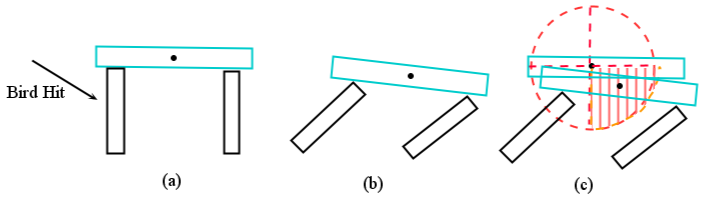
\includegraphics[scale=0.35]{BirdImpact.png}\caption{(a) The object in cyan is supported via one-edge support, and the impending impact is indicated by the arrow (b) A subsequent scene after the bird hit (c) The estimated open quadrant (shadowed area)}
\label{BirdImpact}
\end{figure}

\begin{figure}[h!]
\centering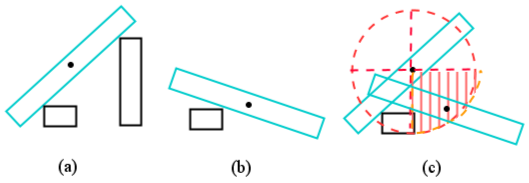
\includegraphics[scale=0.4]{QudrantsEstimation.png}\caption{(a) The right-leaning object (in cyan)  (b) a subsequent scene where the object falls to the right (c) The estimated open quadrant (shadowed area)}
\label{QudrantsEstimation}
\end{figure}




\section{Handling Common Movement by Spatial Reasoning}\label{trackingBySpatialReasoning}

One challenge is to find out a matching between identical objects that are close to each other, and have the similar motions.  

Figure \ref{SCOExample_2}.a  shows a scene where object A and B forms a slope and there are three identical squares $o_1$, $o_2$ and $o_3$ lying on the slope. Figure \ref{SCOExample_2}.b is a subsequent image where the three squares went down a bit. There are 6 ways to match between the squares while only $\{o_1 \sim o_4, o_2 \sim o_5, o_3 \sim o_6\}$ is possible. Without reasoning about  the spatial relations between the squares, some optimization algorithms, e.g. minimizing centroid shift, will tend to match $o_2$ with $o_6$. In many cases, objects dynamics such as velocities are unavailable, thus most of state of the art tracking algorithms do not apply well because of the lack of a suitable dynamic model. 

Human can solve this case efficiently by spatial reasoning. Since we know the objects are moving at the similar velocity, the relative spatial changes among them can be subtle. Hence the spatial relations between those objects can hardly change to the converse as they are moving. When matching, we are trying to keep the original spatial relations among the subsequent objects. 

We emulate this reasoning to test a match in the way that first identify those objects that will follow the similar motion and then check whether a relation changes to the converse in the subsequent image. 

"We observe that objects are likely to follow a common motion if they have the same contact relations with the same objects." [PLEASE EDIT the quoted sentence: i do not know how to say it in the formal way, the basic idea is, if the object contact others via the same contacts relations, then they may be influenced in the similar way since objects interactions are via contacts]. We call such objects as $spatially\,\,correlated\,\,objects$ (SCO). Figure \ref{SCOExample} shows some examples of SCO in a typical angry birds scenario.

Given a set of initial objects, we obtain the SCOs by checking the node equivalence in the corresponding EGSR network. A node is equivalent to another if they hold the same contact relations with the same other nodes. Thus the slope example has only one SCO $\{o_1, o_2, o_3\}$(see Figure \ref{SCOExample_2}.c)

 Having identified the SCOs, we then check the spatial relations between their matched objects in the subsequent image. Formally, let $R$ be a set of EGSR relations, the converse of a relation $r \in R$ is written as $r^{\prime} \in R$. Given a group of spatially correlated objects in the initial image $O = \{o_1, o_2, ... , o_k\}$ and set of subsequent objects $O^\prime = \{o^{\prime}_1, o^{\prime}_2, ..., o^{\prime}_k \}$ with a match $\forall i\leq k, o_i \sim o^{\prime}_i$ between them, the spatial constraints can be written as $\forall o_i,o_j\in O\exists r\in R, o_i \{r\} o_j \Rightarrow o^{\prime}_i \{r^{\prime}\} o^{\prime}_j does\,not\,hold$, $i,j \leq k$. If a match violates the constraints, we will try all the other possible matches among the SCO until the violation is resolved. 

In the slope example, a match $\{o_1\sim o_4, o_3\sim o_5, o_2 \sim o_6\}$ violates the constraint because $o_2\{LEFT\}o_3$, $o_6\{RIGHT\}o_5$ while $RIGHT$ is the converse of $LEFT$

\begin{figure}[h!]
\centering\includegraphics[scale=0.7]{SCOScenario.png}\caption{(a) A typical Angry Birds scenario (b) The corresponding SCOs (highlighted by different color)}
\label{SCOExample}
\end{figure}

\begin{figure}[h!]
\centering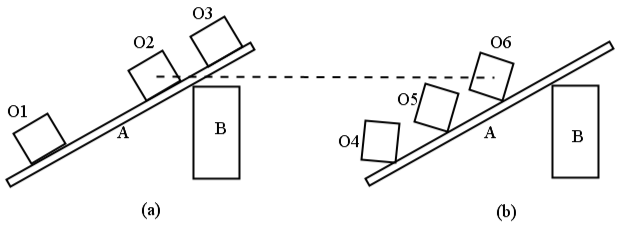
\includegraphics[scale=0.3]{SCOScenario_2.png}\caption{(a) An initial scene (b) A subsequent scene where the squares slide down a bit (c) The EGSR constraint network of the initial scene (only retain the edges indicating contacts) and the SCO}
\label{SCOExample_2}
\end{figure}


\section{A Method for Objects Tracking}
Let $O$ and $O^{\prime}$ be a set of objects in an initial image and a subsequent image taken at a later time, respectively. For ease of notation, we will refer to objects in $O$ as initial objects and objects in $O^{\prime}$ as new objects.

First, the method randomly assigns a unique ID to each initial object, and estimates the MBC quadrants of each object according to the object's spatial relations. The domain for each initial object is set so that it contains only the new objects that are of the same object type and within the MBC quadrants. The method then creates a preference list from the domain of each of the initial objects: the new objects in the preference list are sorted by the size of the centroid shift from the initial object in ascending order. The method matches the two sets of objects using a stable marriage algorithm with the pre-computed preference lists. The algorithm ensures each match is stable in the sense that no pair of objects would prefer each other over their matched partners. 

Then, the method finds all groups of spatially correlated objects among the initial objects and gets their corresponding objects from the match. The method then checks to see whether a spatial constraint has been violated, as mentioned in \ref{trackingBySpatialReasoning}. If there has, it resolves it accordingly.

 

\section{Implementation}
We implemented our method and applied it to the Angry Birds where the vision can detect the exact shapes of the objects\cite{}. The objects' visual appearance are restricted to a finite number of templates (See Figure \ref{Templates}).

The vision has the following limitations: 
\begin{itemize}
\item Damaged objects will be detected as a few separate smaller pieces. (Figure \ref{Fragments}.b) 
\item Debris are not recognized so that one cannot determine whether an object, say a stone, is a real stone or just a debris from a previously destroyed stone. (Figure \ref{Fragments}.a) 
\item Objects occlusion is not handled. Objects can be partially or entirely occluded by debris or other game effects e.g. prompted scores or clouds around the hit point (See Figure \ref{Fragments}.c)
\end{itemize}

\begin{figure}[h!]
\centering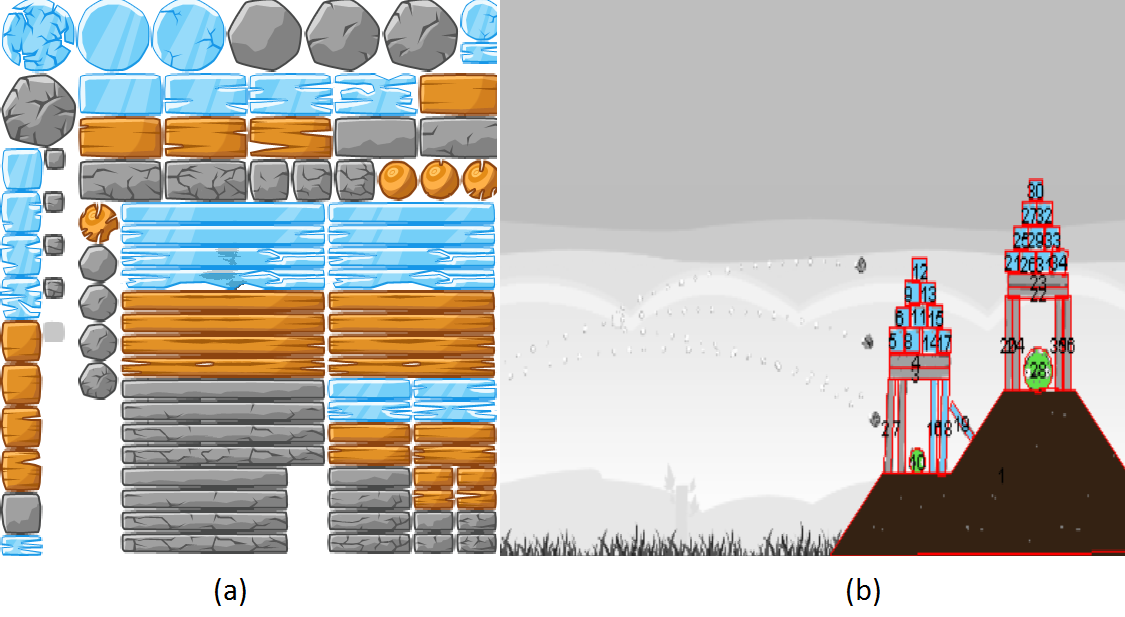
\includegraphics[scale=0.28]{Templates.png}\caption{(a) Main Templates used in Angry Birds (b) The vision detects the real shapes of the objects in a typical Angry Birds scenario}
\label{Templates}
\end{figure}

\begin{figure}[h!]
\centering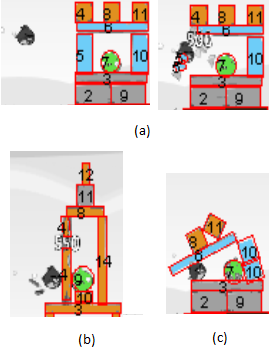
\includegraphics[scale=0.7]{Fragmentation.png}\caption{(a) An object (ID 5) is broken into pieces by a hit (b) An object (ID 4) is partially occluded (c) An object (ID 10) is damaged and detected as two separate blocks}
\label{Fragments}
\end{figure}



\subsection{Handling Fragmentation and Occlusion}

Objects fragmentation creates new objects in subsequent images and the new objects are not directly related to the initial objects. The varying number of objects from one scenario to another can introduce ambiguities making a tracking algorithm off the track. 

In angry birds, the fragmentation is mainly due to objects destruction, partially occlusion, and damage. Handling fragmentation is important. By recognizing the fragments, we are able to infer whether an object is destroyed, damaged, or occluded, which leads to a robust tracking.

We deal with the fragmentation by first recognizing potential fragments, then construct all the possible objects from the fragments, and add them to the pool of the subsequent objects for matching, and finally apply a debris recognition process for the unmatched initial objects. 

To obtain the potential fragments, we group the initial and subsequent objects according to their templates, respectively. If a group of the subsequent objects contains more objects than its initial counterpart, we treat all those subsequent objects as potential fragments.  

For all the potential fragments, we put those that can form a shape of one of the templates into a same group. The shape formed by the group of fragments is an oriented minimum bounding rectangle (OMBR) that bounds all the fragments (see Figure \ref{OMBRs}.a). The fragments from one group must have the same type. We then treat the OMBR as one object in the subsequent image, which can be potentially matched with one of the initial objects. Once the OMBR is matched, all the fragments from the corresponding group are also matched. i.e. assigned with the same ID. In some rare cases, a fragment can be involved in more than one OMBRs. So we add an additional constraint: all the matched OMBRs should not have a common fragment. 

We label unmatched fragments as debris. Destruction of an object will create a cluster of debris around the object's location. Those debris can be of any shape, e.g. circle, polygon and will diffuse until disappear after 2-4 seconds. Given an object $o$ in the initial scenario, we start the debris recognition process if there are no subsequent objects can be matched with $o$ (including the OMBRs created from the fragments). We first draw the MBC of $o$, and get the set of the subsequent objects falling in the MBC excluding those which have been matched. The set of the objects are labelled as debris of $o$ and $o$ is marked as destroyed (see Figure \ref{OMBRs}.b). 

In some cases, an object can be totally occluded for a subsequence of images. To deal with this, before a matching, we cache the spatial configurations of all the initial objects. At the end of the matching, we update the cache by replacing each initial object's configuration with the matched subsequent object's so that the cache always maintains the latest configuration of each initial object. If an occluded object recurs in one subsequent image, we match the occluded object by searching through the cache for an unmatched initial object. The occlude object will be matched if it lies in the MBC of that initial object. 


\begin{figure}[h!]
\centering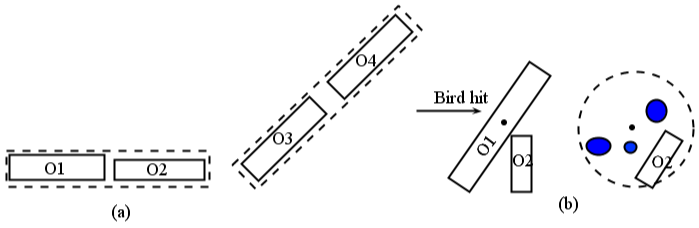
\includegraphics[scale=0.3]{OMBRs.png}\caption{(a) OMBRs are indicated by the dotted rectangles (b) $o_1$ has been destroyed by a bird hit, and the blue dots are recognized as debris}  
\label{OMBRs}
\end{figure}


  
\section{Evaluation}

We measure the accuracy of the tracking method by the number of mismatches, and the percentage of correct matches out of the total number of possible mismatches. 

Specifically, given a set $n$ of objects in an initial scenario and assume $m$ of them are of unique type, the total number of possible mismatches is $n - m$. We count the correct matches $c$ of the $n - m$ objects. The accuracy is  $c / (n - m)$.


The evaluation has been done in two steps. In the first step, we collect samples from active angry birds scenarios, and obtain the ground truth by applying our method using the smallest time gap.

In the second step, we evaluate the method by varying the time gaps and obtain the accuracy by comparing against the ground truth.

 
\subsection{Obtaining Ground Truth}

We collect a sample by capturing a sequence of screenshots before and after a shot using the smallest time gap (50 ms). The average time gap between the beginning and the end screenshot is 10 seconds. i.e. A sample contains around 200 screenshots.  

We apply our method on the whole sequence so that the method will keep tracking the objects through all of the screenshots, from the first until the last (see Figure.\ref{Tracking}). The match between the initial objects in the first screenshot and the subsequent objects in the last screenshot will be saved as ground truth for later evaluation. 

\begin{figure}[h!]
\centering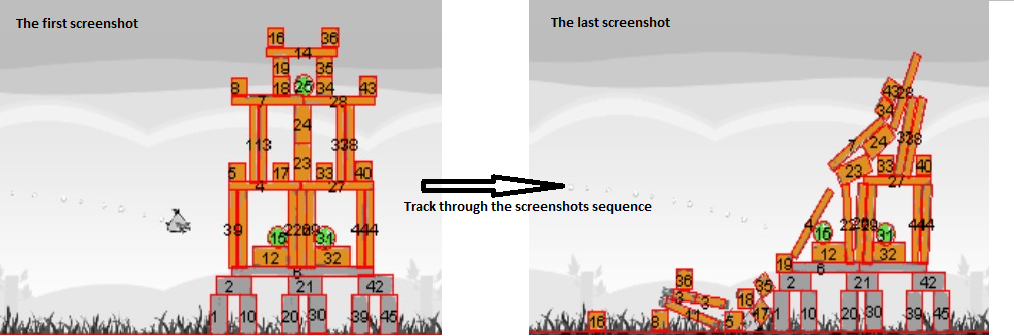
\includegraphics[scale=0.32]{TrackingBackup.png}\caption{The method tracks through the screenshots and label the matched objects with the same ID. The match between the first and last screenshots is saved as the ground truth }
\label{Tracking}
\end{figure}

To automate this process, we run an angry birds agent that always aims at an random pig on the first 21 Poached Eggs Levels \cite{AngryBirdsLevels}. The agent starts to capture screenshots once a shot is made, and stops after 10 seconds. In each level, the agent records the screenshots of at most four shots.

In the end, we have around 80 samples. To evaluate the accuracy of the \"ground truth\", we run our method on 10 samples randomly picked from the 80. We get the accuracy by manually labelling the initial objects and their correspondence in the end screenshot, and compare with the matching. 

It turns out that the method can match most of the objects with less than 5 mismatches per sample. The average time computation is 3.5 ms per match. We then modify the method (denote as $BASIC$) such that it only matches by visual appearance and minimizing the centroid shift between initial and subsequent objects. We compare the results in Table \ref{empiResults}
\begin{table}
\caption{Results on the 10 samples(\,$QSR$: the proposed method $BASIC$: the modified method )}\label{empiResults}
\centering
\begin{tabular}{c|c|c|c|c}
\hline
{} & \multicolumn{2}{c}{Accuracy} & \multicolumn{2}{c}{Mismatch}\\
\hline
Sample & QSR & BASIC & QSR & BASIC \\
\hline
1& 0.95 & 0.70 & 2 & 12\\
2&1.00 & 1.00 & 0 & 0\\
3&0.92 & 0.70 & 4 & 16\\
4&0.93 & 0.89 & 2 & 4\\
5&0.91 & 0.77 & 4 & 10\\
6&1.00 & 0.95 & 0 & 2\\
7&1.00 & 0.91 & 0 & 2\\
8&0.93 & 0.80 & 2 & 6 \\
9&0.93 & 0.80 & 2 & 6\\
10&0.92 & 0.85 & 2 & 4\\
\hline
\end{tabular}
\end{table}

\subsection{Experimental Results}

We evaluate our method on the 80 samples with varying time gaps, namely 100 ms, 200 ms (the maximum delay in getting screenshot from the server used in Angry Birds AI competition), 300 ms (the time taken by requesting a screenshot plus the vision segmentation) and 1000 ms

For a particular time gap of size $T$, the method will track through every $T/50$ screenshots from the original sequence. The accuracy and mismatch is obtained by comparing against the saved ground truth. As expected, the accuracy drops down when applying larger time gaps (see Table \ref{empiResults_2}).  

\begin{table}
\caption{Results on the 80 samples with different time gaps}\label{empiResults_2}
\centering
\begin{tabular}{c|c|c|c|c}
\hline
Time gap (ms) & Average Accuracy & Average Mismatch \\
\hline
100 & 0.93 & 2.05\\
200 & 0.89 & 3.22\\
300 & 0.88 & 3.4\\
500 & 0.85 & 3.98\\
1000 & 0.84 & 4.1\\
\hline
\end{tabular}
\end{table}




\section{Conclusion and Future Work}
\begin{algorithm}[!]
\caption{The Object Tracking Algorithm}\label{algo}
\begin{algorithmic}[1]
\Procedure {MatchObjects}{$objs$}
\State $iniobjs$ //initial objects
\State $solution \leftarrow \{iniobjs, \{\}\}$
\State $domain \leftarrow \{\}$// A map stores each initial object and a list of possible correspondence 
\State $domain \leftarrow$ MotionApproximation($objs$) 
\State CalculatePreference($iniobjs$, $domain$) //Calculate the preference list of $iniobjs$
\State $freeobjs \leftarrow iniobjs$
\While{$freeobjs$ is not empty}
\State $iniobj \leftarrow freeobjs.pop()$
\State get a next preferred $obj$ from $iniobj$'s preference list  
\If {$obj$ is not assigned yet}
  \State match($iniobj$, $obj$)
  \Else{$obj$ has been assigned to $iniobj^{\prime}$}
  \If{$obj$ prefers $iniobj$ to $iniobj^{\prime}$}
  \State match($iniobj$, $obj$), add $iniobj^{\prime}$ to $freeobjs$
\EndIf 
\EndIf
\EndWhile
\State $cobjsList \leftarrow$ GetSCO($objs$)// get spatially correlated objects
\State SPC($solution$) //Spatial Constraints Check
\State $iniobjs \leftarrow objs$
\EndProcedure

\Procedure{GetSCO}{$objs$}
\State $cobjsList \leftarrow \{\}$
\For {$obj \in objs$}
\State $cobjs \leftarrow objs$ 
\State $tobjs \leftarrow$ a set of the objects that touch $obj$
\For {$tobj \in tobjs$}
\State $ttobjs \leftarrow$ a set of the objects excluding $obj$ that touch $tobj$ via the same contact relation.
\State $cobjs \leftarrow cobjs \cap ttobjs$
\EndFor
\State $cobjsList \leftarrow cobjsList \cup cobjs$
\EndFor
\Return $cobjsList$
\EndProcedure
\Procedure{MotionApproximation}{$objs$}
\For {$obj \in objs$}
\State $domain \leftarrow domain \cup \{obj, \{\}\}$
\State $pobjs \leftarrow \{\}$
\State compute the MBC of $obj$
\State analyse the stability of $obj$ according the rules specified in \ref{} and locate the corresponding quadrants.
\State Remove the objects which are of different type, and add the remaining objects in the quadrants to $pobjs$. 
\State $domain \leftarrow domain \cup \{obj, \{pobjs\}\}$
\EndFor
\Return $domain$
\EndProcedure
\Procedure{Match}{$iniobj$, $obj$}
\State $obj.id \leftarrow iniobj.id$, $solution \leftarrow \{iniobj, obj\}$
\EndProcedure
\Procedure{SPC}{$solution$}
\For {$cobjs \in cobjsList$}
\State for each object in $cobjs$, get its matched $obj$ from $solution$
\State Check whether the spatial constraints \ref{} are violated. If violated, re-assign the objects until violation is resolved  
\EndFor
\EndProcedure
\end{algorithmic}
\end{algorithm}
 \end{document}